\subsection*{ГЛ13 2}
 Заметим, что пучок коник -- это прямая в $\mathbb{P}_5$. Рассмотрим отображение
\begin{equation*}
	\upvarphi: L \rightarrow b_4^\times 
\end{equation*}
Оно является гомографией, так как биективно и рационально. \\
Гомография переводит конику в касательную прямую в точке $b_4$.\\
При гомографии двойное отношение не меняется: $[b_4b_1, b_4b_2, b_4b_3, b_4b_4]_{b_4^\times}=[S_1, S_2, S_3, C]_L$, так как $b_4b_4=t$\\ 
\begin{figure}[h!]
	\center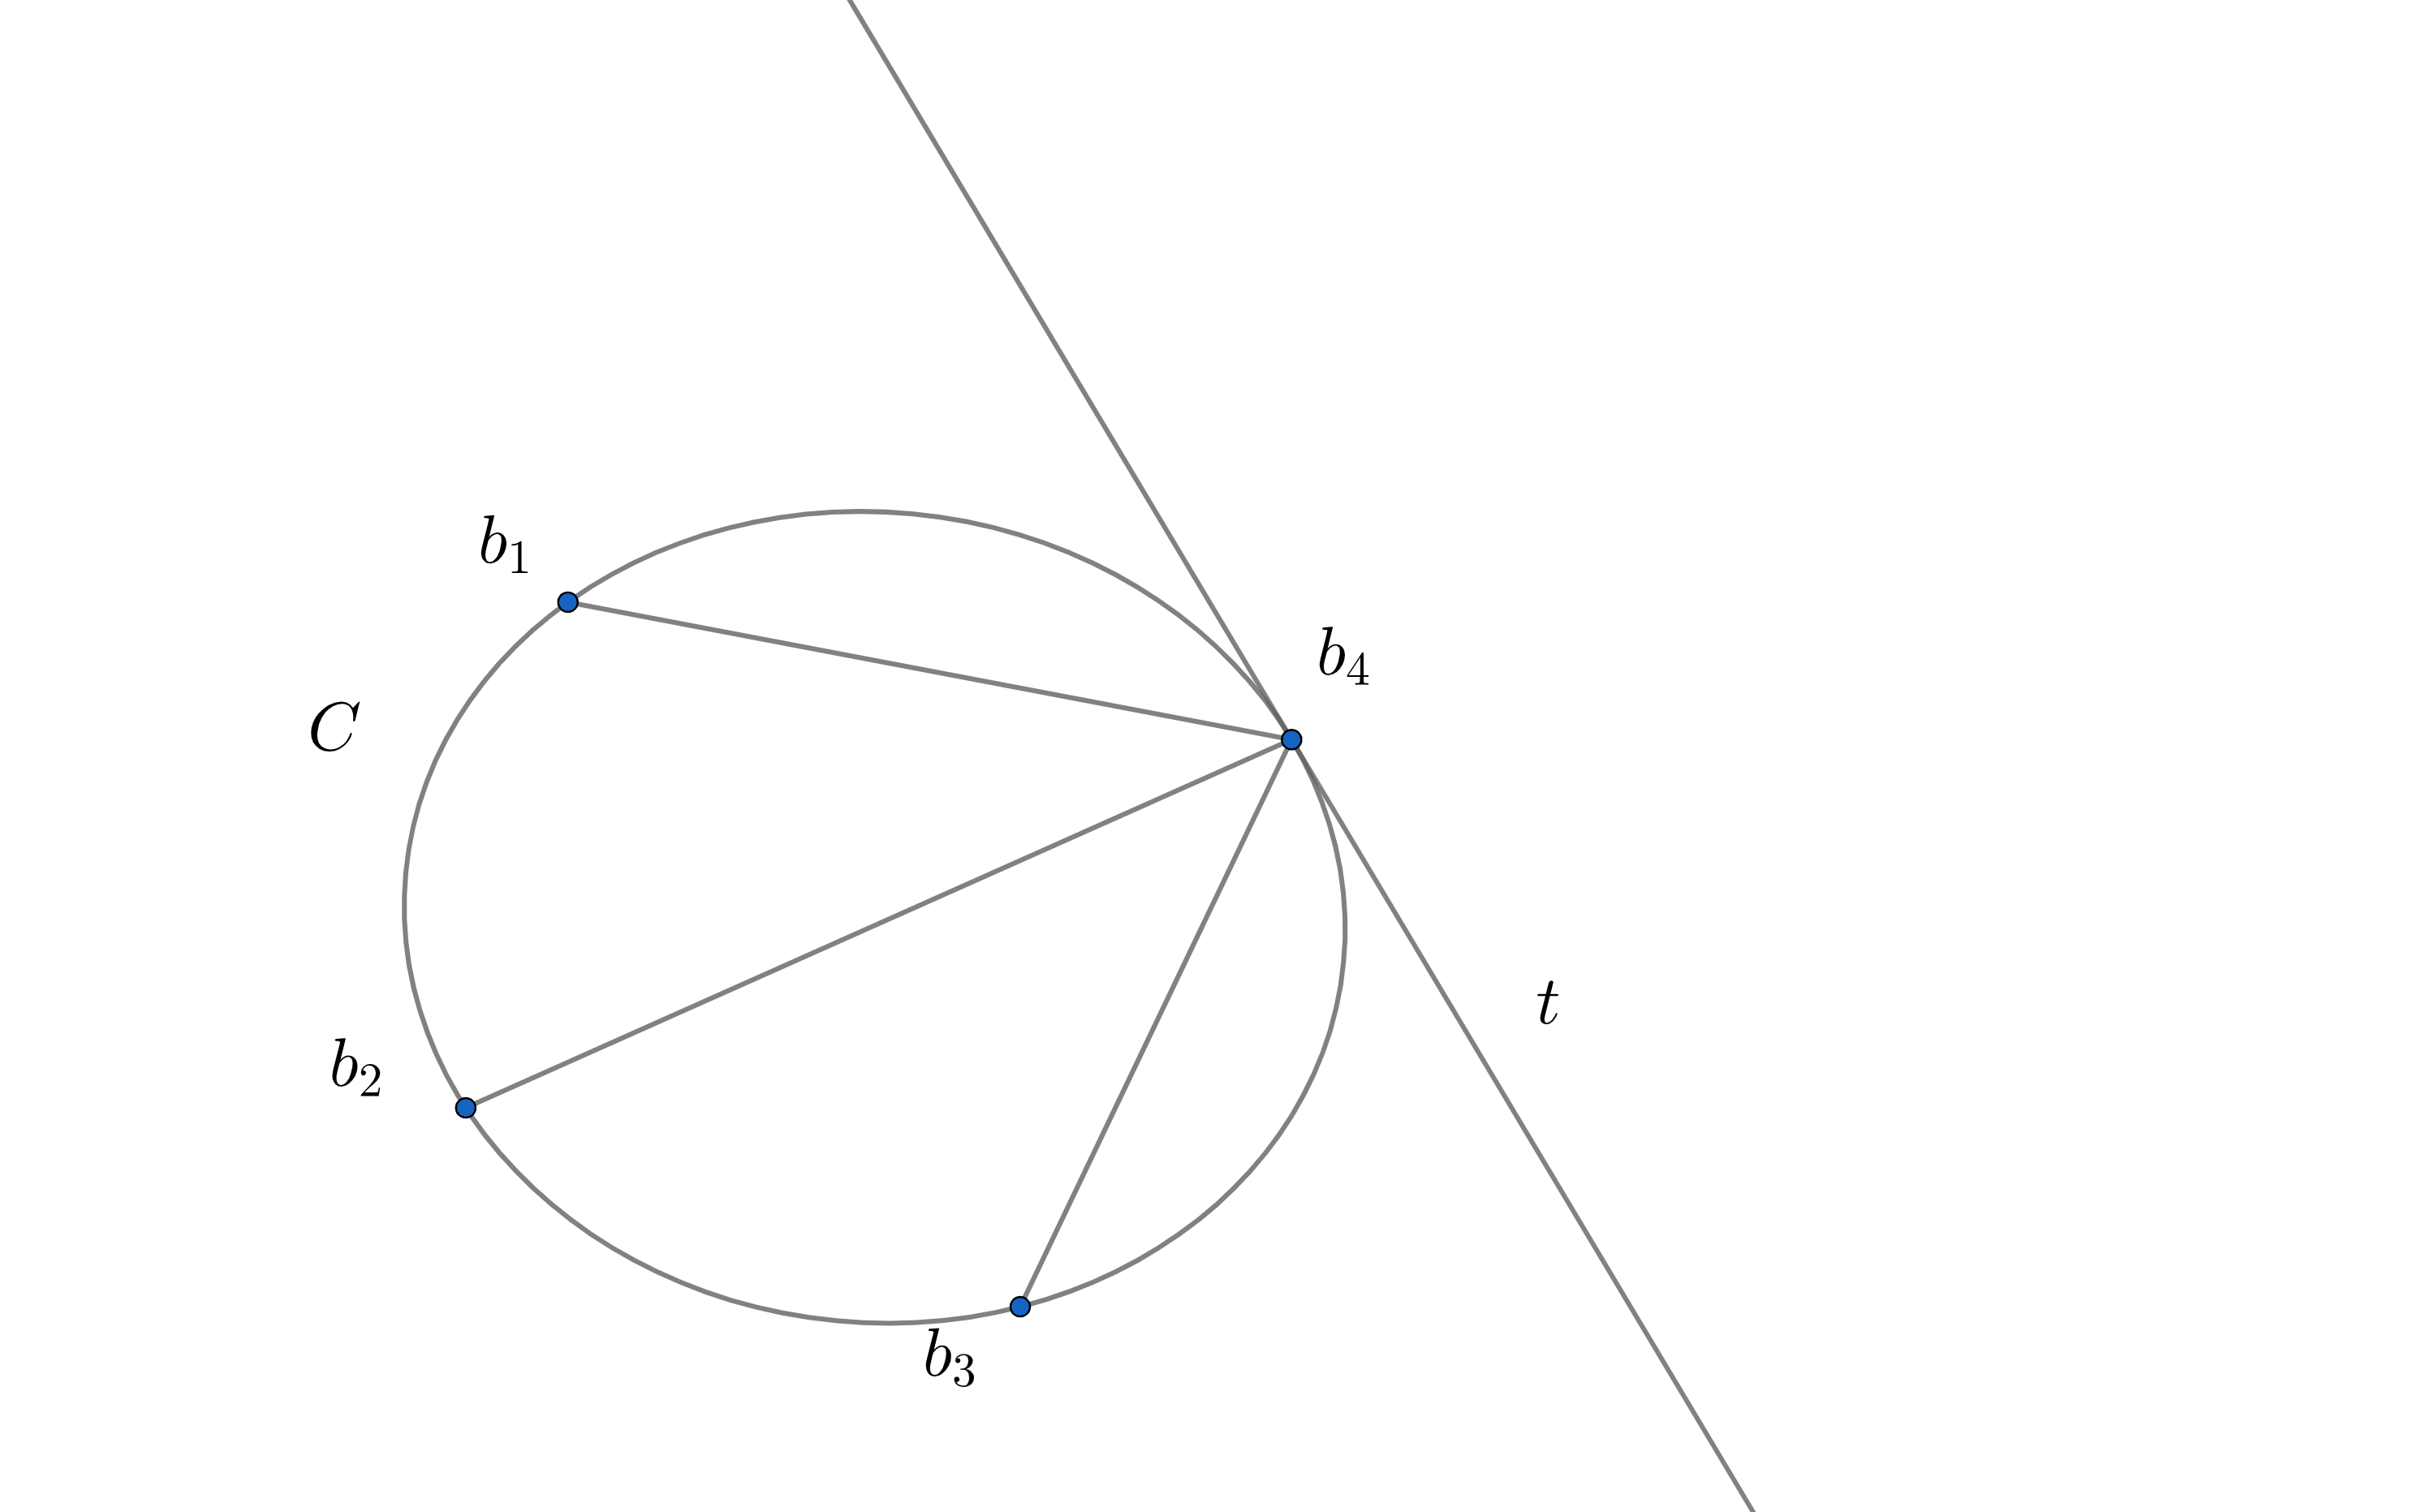
\includegraphics[width=0.6\linewidth]{pic28}
\end{figure}\\
По определению   $\left[b_{1}, b_{2}, b_{3}, b_{4}\right]_C=[pb_1, pb_2, pb_3, pb_4]_{p^\times}$, где $p \in C$ \\
Если $p=b_4$, то $\left[b_{1}, b_{2}, b_{3}, b_{4}\right]_C=[b_4b_1, b_4b_2, b_4b_3, b_4b_4]_{b_4^\times}=[S_1, S_2, S_3, C]_L$\\